\section{Problem Formulation}
\label{sec:problem_statement}

In this paper, we target heterogeneous MPSoCs that consist of
customizable Processing Elements (PEs), which can be realized with the
use of ASIPs. Each PE has private cache and communicates with other PEs
via dedicated communication buffers (for example, FIFO queues). Each
PE can be customized by both extending its baseline instruction set
architecture and customizing its cache. Additionally, each PE can operate
in several discrete voltage and frequency levels. Thus, the heterogeneity
in the MPSoC is manifested in terms of custom instructions, custom cache
configurations and voltage/frequency levels.

The target application domain comprises of streaming applications, which
contains multiple compute-intensive sub-kernels or tasks. The task graph
of an application is a directed acyclic graph, where the tasks are
mapped to PEs to enable pipelined execution of the streaming application. 
Figure~\ref{fig:pipeline} illustrates the pipelined execution in MPSoC. For example, two tasks are mapped to the first PE and one task is mapped to the second PE. The PEs form the logical stages of the pipeline. At the end of each stages of the pipeline, a single iteration of a task is completed. The steady state in the given example is reached after the stage one of the second PE. The period of the pipeline is defined as the maximum latency among all the stages (as shown in Figure~\ref{fig:pipeline}. 

Each task can be accelerated with a set of custom instructions. Hence, there are multiple
implementations of each task corresponding to differing sets of custom
instructions that can be used. Each set of custom instructions for a
task is associated with its additional area. Furthermore, each task can
be executed with one of the available discrete voltage and frequency
levels. The execution time and energy consumption of a task then depends
on the cache configuration of the PE on which it is mapped, and the set
of custom instructions and voltage/frequency level selected for it. The
area of the baseline PE, additional custom instructions and the cache
configuration determines the total area of the PE. The area of the
MPSoC is then the summation of the area of all the PEs.

Benoit et al.~\cite{general_mapping} categorizes the policies to map tasks of a task
graph on an MPSoC with fixed number of PEs into: one-to-one mapping,
where only a single task is mapped to a PE; interval based mapping, where
only adjoining tasks are mapped to a PE; and, general mapping, where no
restrictions are placed at all. In this paper, we use general mapping
which offers greater flexibility, and has the potential to reach better
global optima. In summary, our design space exploration should
search through: a) the number of PEs, b) mapping of the tasks on the
the PEs, c) the cache configurations for each of the PEs, d) the sets of
custom instructions for each of the tasks , and e) the voltage/frequency
levels for each of the tasks.

The problem can be formally stated as follows: given an acyclic task
graph of an application, differing sets of custom
instructions for each task, differing discrete voltage/frequency levels
for each task, differing cache configurations for a PE, the steady state
period constraint and the area constraint, the goal is to minimize the
total energy consumption of the MPSoC. Therefore, the following need to
be determined:
\begin{itemize}
\item The energy-wise optimal number of PEs and mapping of the tasks on them.
\item The energy-wise optimal cache configuration for the each of the
individual PEs.
\item The energy-wise best set of custom instructions and voltage/
frequency level for each task.
\end{itemize}

Note that the optimization problem described above cannot be solved
naively because of its exponential complexity, which results from all
the possible combinations of task mapping, cache configurations, sets of
custom instructions, and voltage/frequency levels.


\begin{figure}[h]
\center
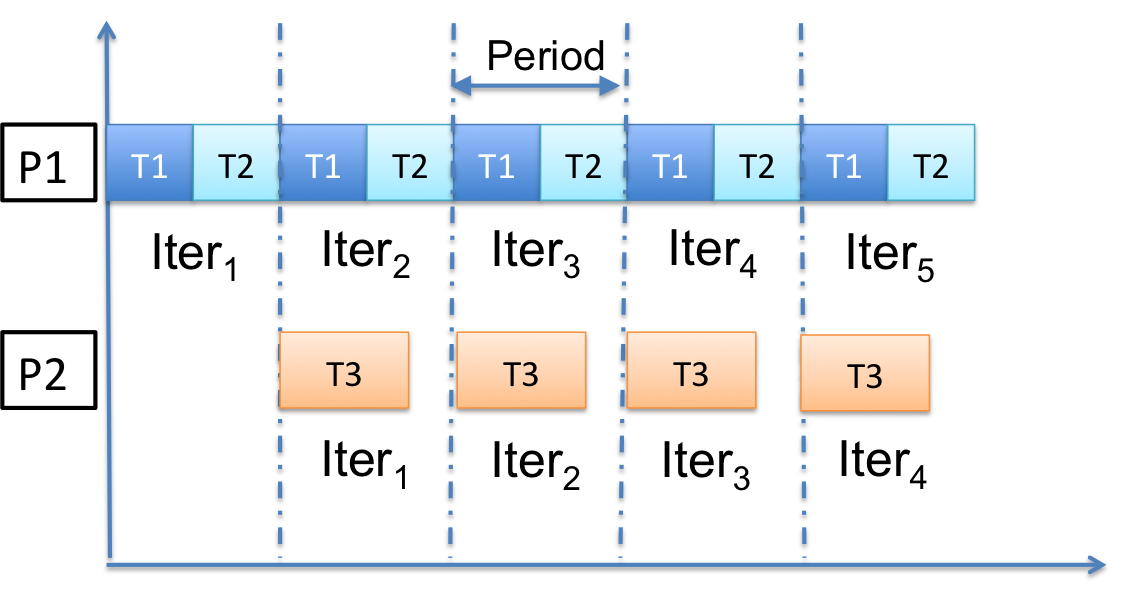
\includegraphics[scale=0.40]{pipeline.png}
\label{fig:pipeline}
\caption {Pipelined Execution}
\end{figure}
